\points{4a} \textbf{Sampling using Vanilla DDPM and DDIM}

For \href{https://arxiv.org/pdf/2006.11239}{DDPM}, the posterior distribution of $x_{t-1}$ given $x_t$ and $x_0$ is known:
\[
    q(x_{t-1} \mid x_t, x_0) = \calN(x_{t-1}; \tilde{\mu}_t, \tilde{\beta}_t I),
\]
with
\[
    \tilde{\mu}_t = \frac{\sqrt{\bar{\alpha}_{t-1}}\beta_t}{1-\bar{\alpha}_t} x_0 
    + \frac{\sqrt{\alpha_t}(1-\bar{\alpha}_{t-1})}{1-\bar{\alpha}_t} x_t,
\]
and
\[
    \tilde{\beta}_t = \frac{1-\bar{\alpha}_{t-1}}{1-\bar{\alpha}_t}\beta_t.
\]

By iterating these steps backward from $T$ to $0$ and adding Gaussian noise at each step (except $t=0$), we reconstruct a clean sample from pure noise.

Given the provided code in the \texttt{sample.py} file, please implement the following functions:

\begin{itemize}
    \item \texttt{get\_timesteps}
    \item \texttt{predict\_x0}
    \item \texttt{compute\_forward\_posterior\_mean}
    \item \texttt{compute\_forward\_posterior\_variance}
\end{itemize}

To generate mnist sample run: 
\begin{lstlisting}[language=bash]
    python run_sampling.py --dataset mnist --experiment ddpm
\end{lstlisting}

Run the experiment to generate few samples with \textbf{num\_steps}=5, 10, 20, 50 and provide a comment. 
\textbf{Hint: }Once we stabilize the quality at 10, we notice that the result is always almost the same.

If you have enough time and resources you can run to generate 256x256 faces samples

\begin{lstlisting}[language=bash]
    python run_sampling.py --dataset faces --experiment ddpm
\end{lstlisting}

You will generate samples thast look like:

\begin{figure}[h]
    \centering
    
\includegraphics[width=0.5\textwidth]{./figures/ddpm_steps1000_seed42_img_0}
    \caption{DDPM samples for Celebrity dataset}
\end{figure}

\textbf{DDIM Sampling}

DDIM sampling provides a shortcut:
\[
x_{t-1} = \sqrt{\bar{\alpha}_{t-1}}x_0 + \sqrt{1-\bar{\alpha}_{t-1}}\epsilon_\theta(x_t,t).
\]
This is a special case of the general formula (16) in \href{https://arxiv.org/pdf/2010.02502}{the DDIM paper} where $\eta = 0$.

Run the \texttt{ddim\_inference} to implement the DDIM update following the previous equation.

To generate mnist sample run: 
\begin{lstlisting}[language=bash]
    python run_sampling.py --dataset mnist --experiment ddim
\end{lstlisting}

Run the experiment to generate few samples with \textbf{num\_steps}=5, 10, 20, 50 and provide a comment. 
\textbf{Hint: }Once we stabilize the quality at 10, we notice that the result is always almost the same.

If you have enough time and resources you can run to generate 256x256 faces samples

\begin{lstlisting}[language=bash]
    python run_sampling.py --dataset faces --experiment ddim
\end{lstlisting}

You will now generate samples thast look like:

\begin{figure}[H]
    \centering
    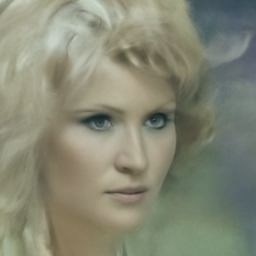
\includegraphics[width=0.5\textwidth]{./figures/ddim_steps10_seed42_img_0}
    \caption{DDIM samples for Celebrity dataset}
\end{figure}